\chapter{Collision SPH}
\label{chap:csph}

We model the collision between elastic solids using a penalty-based contact
force model. A contact force based approach for collision handling
eliminates the spurious interaction between bodies, which occurs while modeling
with an SPH-based model. The contact force model follows the work of
\textcite{mohseni2021particle}.

We demonstrate in \cref{fig:de-stress-wave-compare}, the abilities of the
developed solver in handling the collision between multiple elastic solids by
simulating the elastic wave propagation in a granular media. We consider five
identical disks placed at an angle of $45$ degrees, which are allowed to be
impacted by a moving wall from right with a velocity $5.6$
m\,s\textsuperscript{-1} in horizontal direction.
\begin{figure}[tpb]
  \centering
  \begin{subfigure}{0.8\textwidth}
    \centering
    \includegraphics[width=0.7\textwidth]{images/csph/images/de_2021_stress_wave_in_granular_material_part_2/bardenhagen_2001}
    \subcaption{}\label{fig:de-stress-wave-bardenhagen}
  \end{subfigure}

  % \begin{subfigure}{0.8\textwidth}
  %   \centering
  %   \includegraphics[width=0.7\textwidth]{images/csph/images/de_2021_stress_wave_in_granular_material_part_2/tlmpm_2021}
  %   \subcaption{}\label{}
  % \end{subfigure}

  \begin{subfigure}{0.8\textwidth}
    \centering
    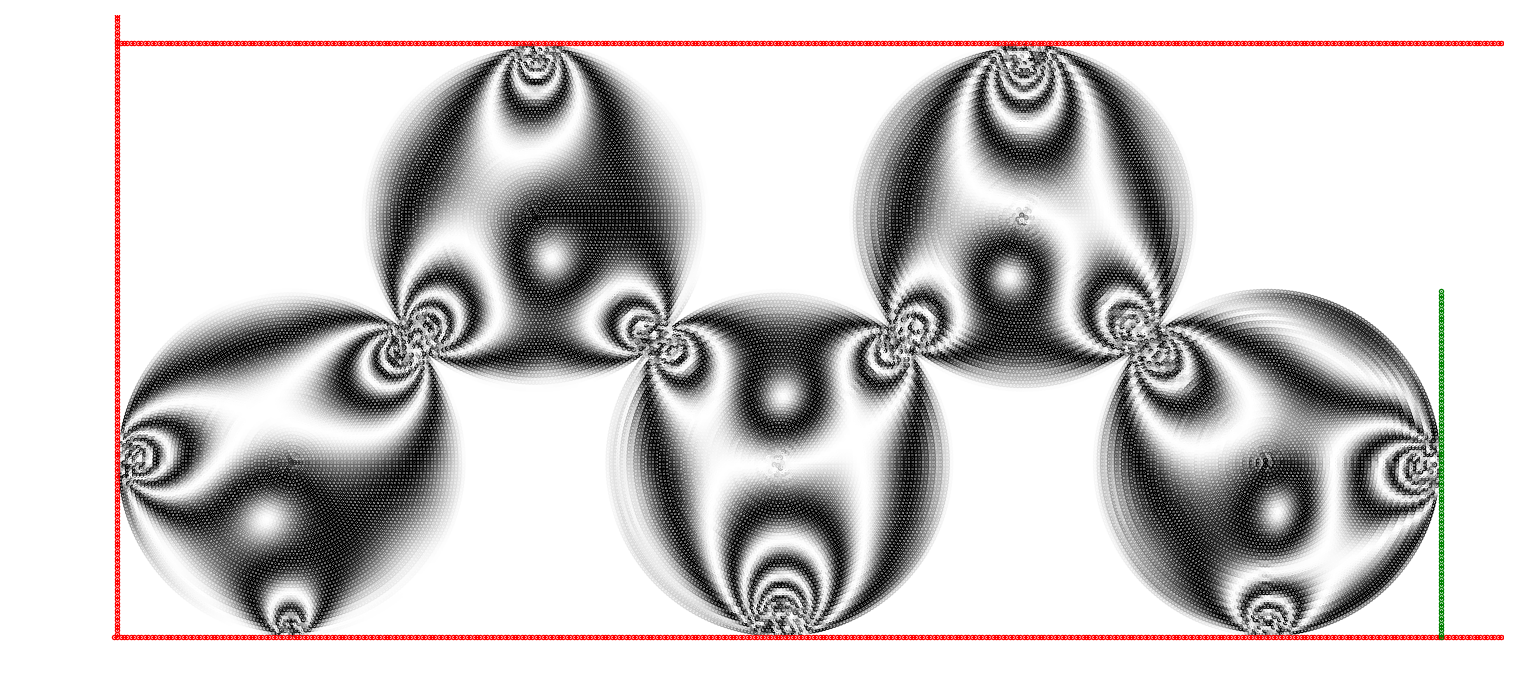
\includegraphics[width=0.8\textwidth]{figures/csph/figures/de_2021_stress_wave_in_granular_material_part_2/case_mohseni/time0}
    \subcaption{}\label{fig:de-stress-wave-current}
  \end{subfigure}
  % \caption{Stress fringes of the granular discs from (a) experiment
  %   \citep{guilkey2001improved}, (b) TLMPM \citep{de2021modelling} (c) Current work}
  \caption{Stress fringes of the granular discs from (a) experiment
    \citep{guilkey2001improved}, (b) Current work}
\label{fig:de-stress-wave-compare}
\end{figure}




We apply the developed solver to model the large deformation of
solids. We consider the collision between two elastic rubber rings. The rings
are made up of a density of $1200$ kg\,m\textsuperscript{-3}, Young's modulus
$E$ of $10$ MPa, and a Poisson's ratio $\nu$ of $0.47$. The evolution of the
colliding rings is shown in \cref{fig:rings:new-ipst-nu-0-47}. From
\cref{fig:rings:new-ipst-nu-0-47} we can say that the current solver is able to
model the collision between elastic solids successfully.
\begin{figure}[tpb]
  \centering
  \begin{subfigure}{0.48\textwidth}
    \centering
    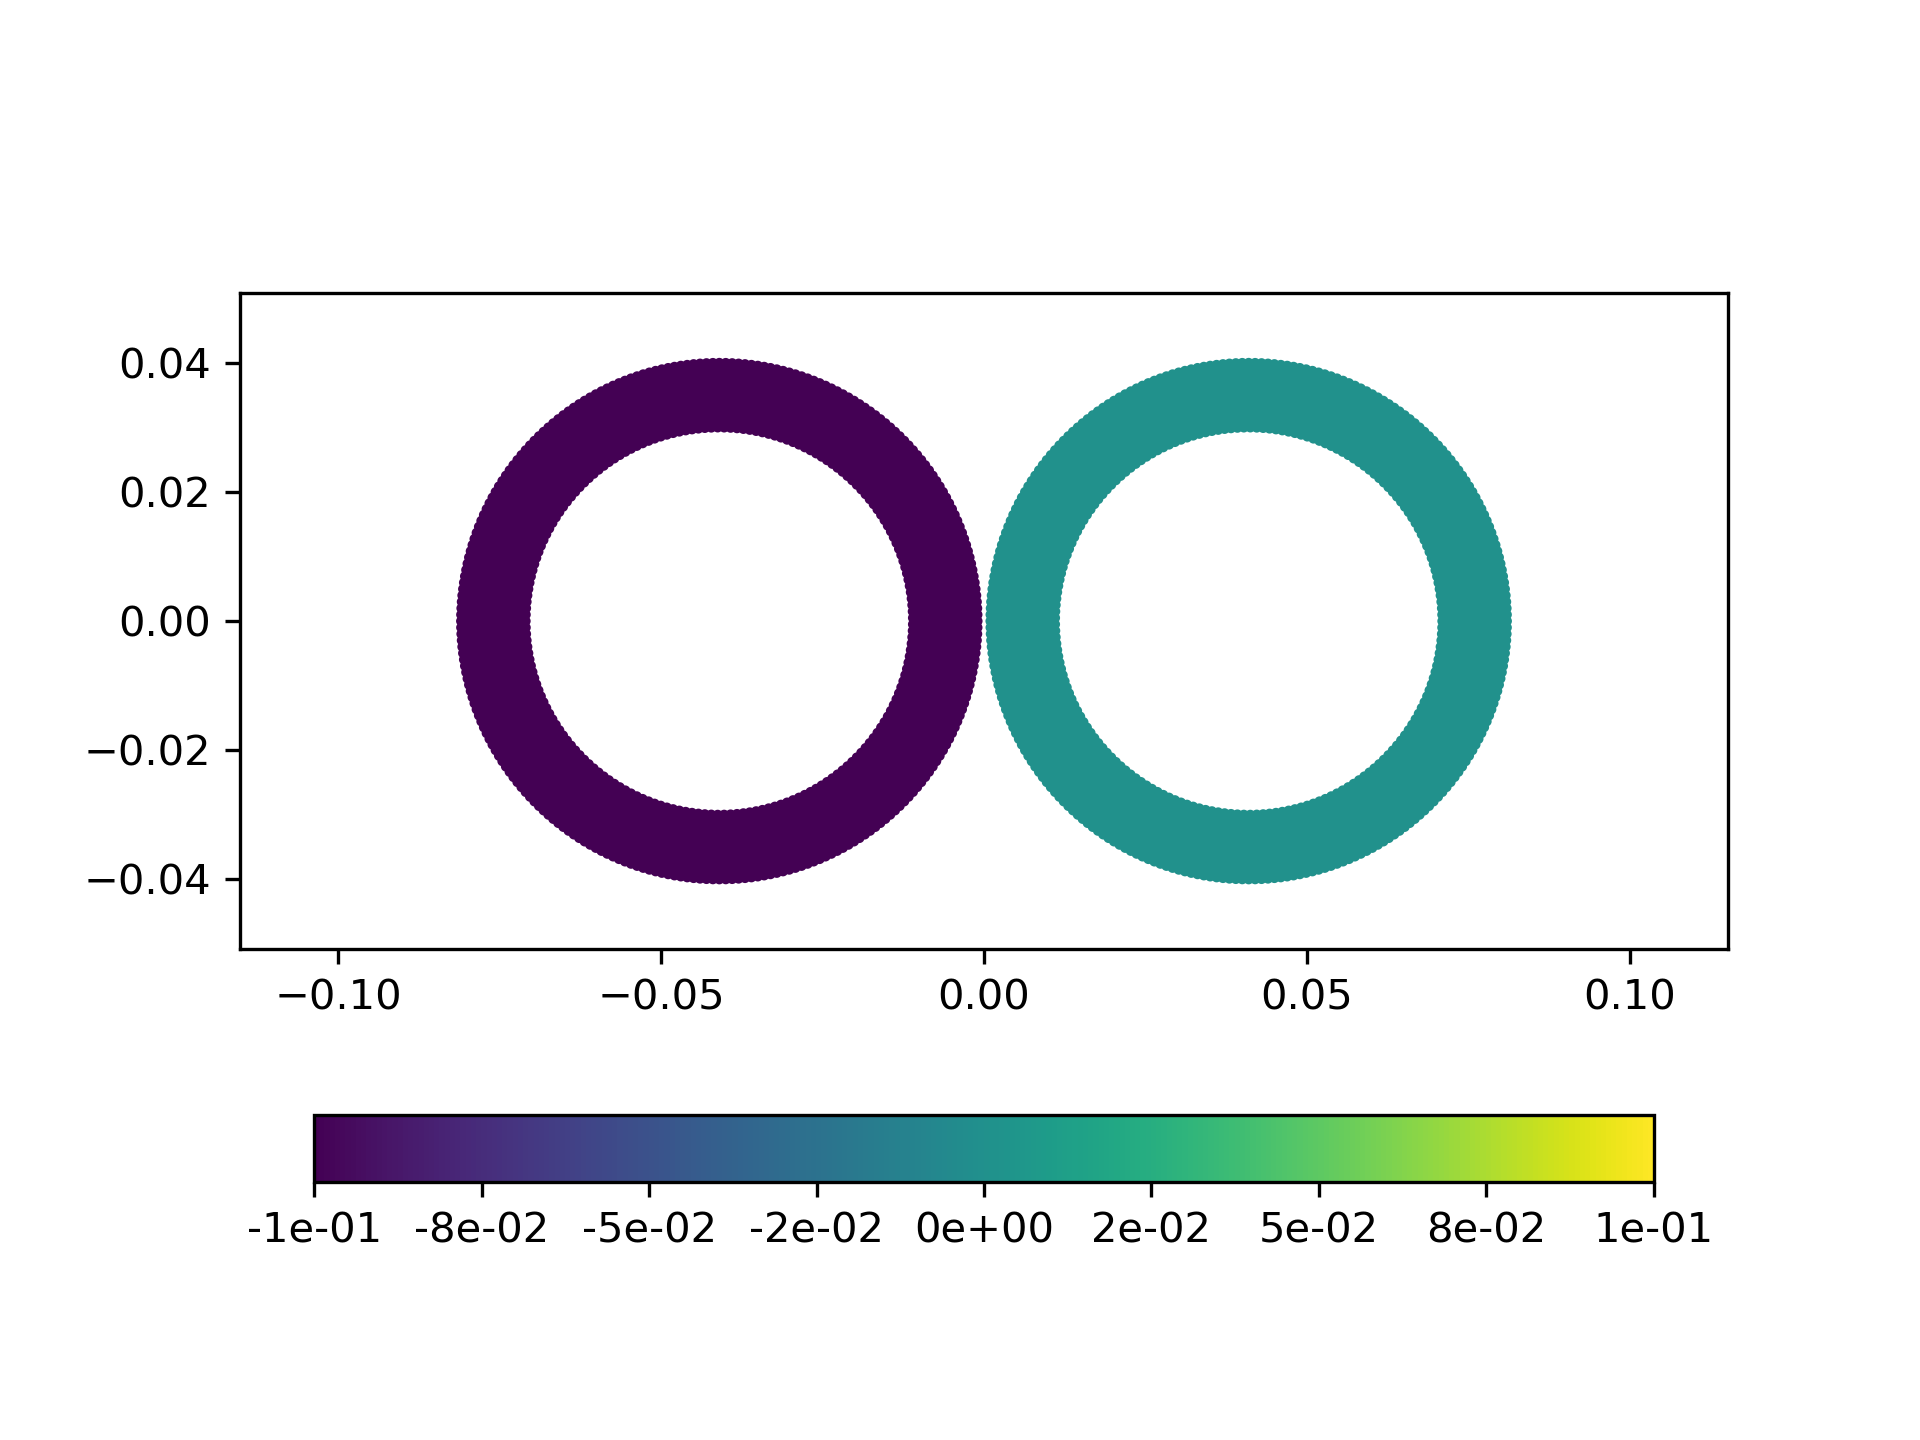
\includegraphics[width=1.0\textwidth]{figures/csph/figures/yan_2021_colliding_rubber_rings/poisson_ratio_0_47/time0}
    \subcaption{t = $0$ ms}\label{fig:rings:ipst-nu-0.47-1}
  \end{subfigure}
  %
  \begin{subfigure}{0.48\textwidth}
    \centering
    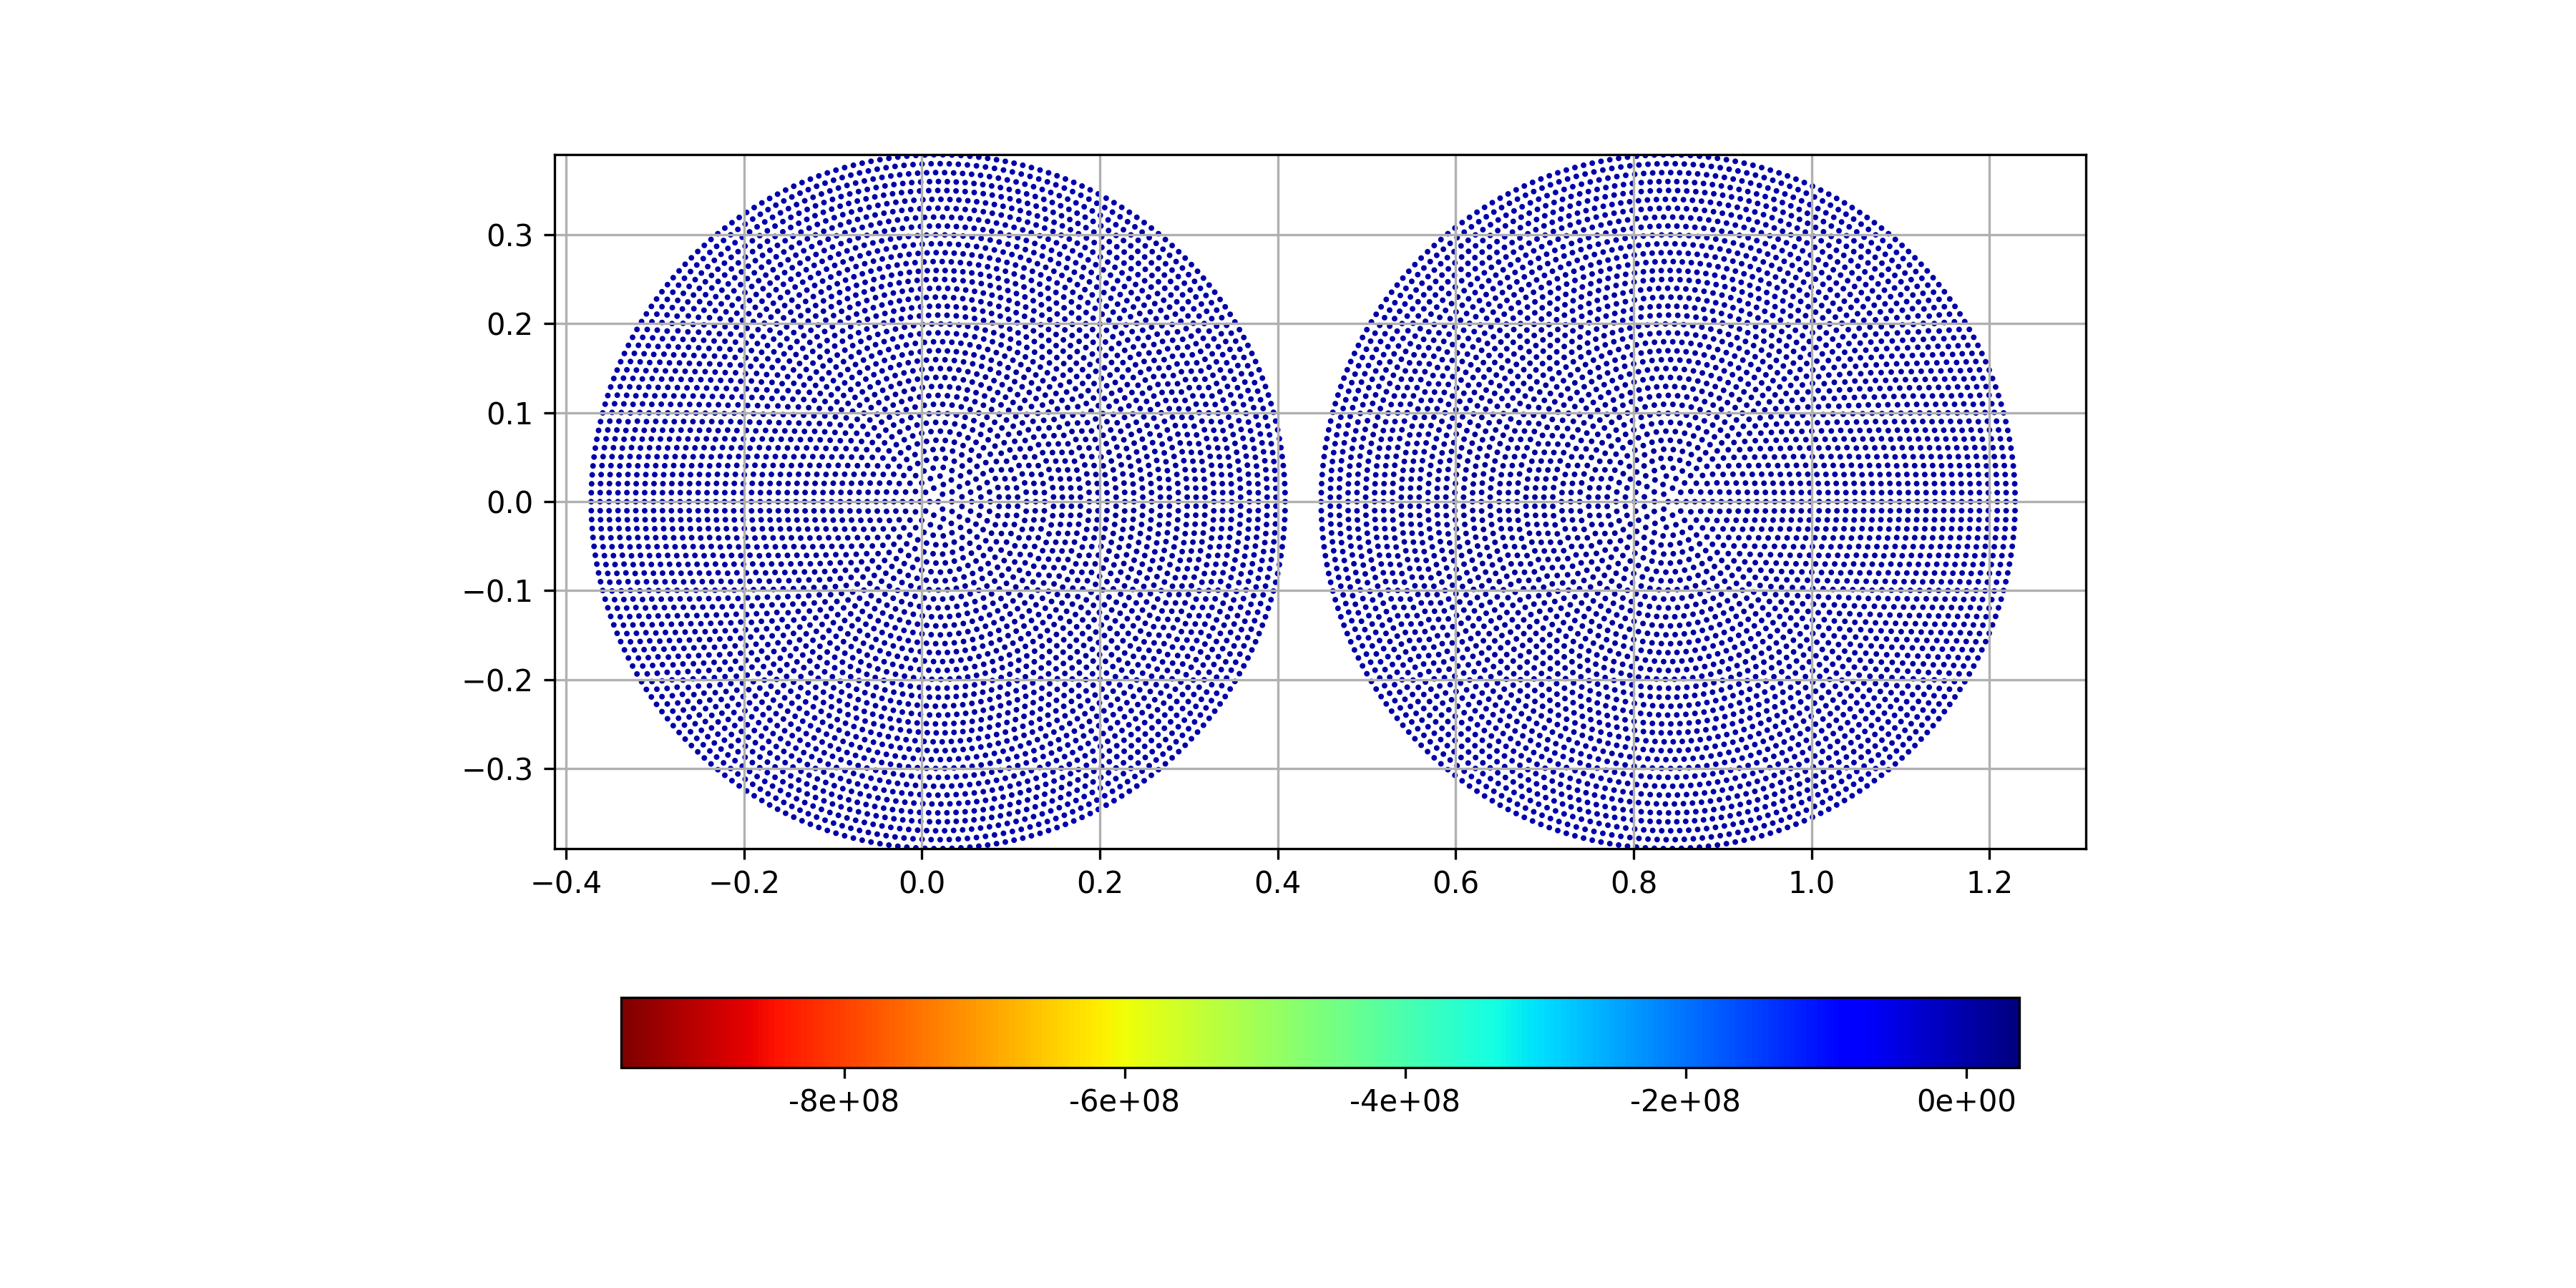
\includegraphics[width=1.0\textwidth]{figures/csph/figures/yan_2021_colliding_rubber_rings/poisson_ratio_0_47/time2}
    \subcaption{t = $5.17$ ms}\label{fig:rings:ipst-nu-0.47-3}
  \end{subfigure}

  \begin{subfigure}{0.48\textwidth}
    \centering
    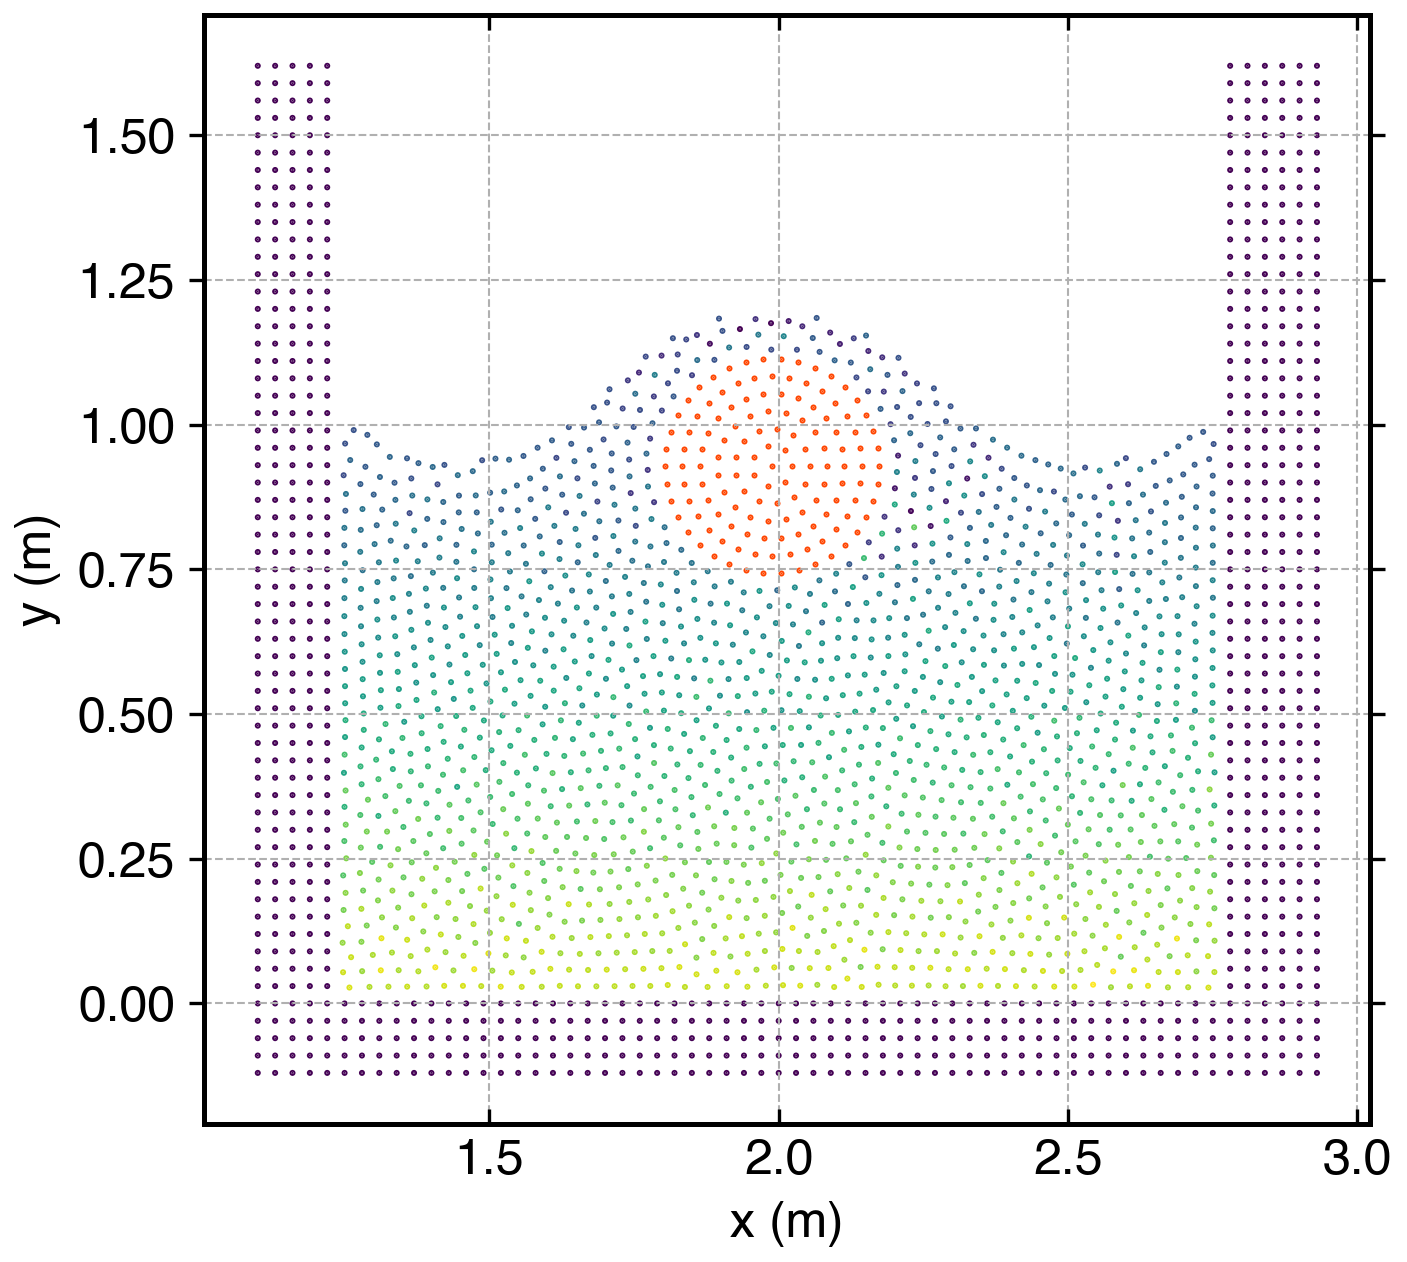
\includegraphics[width=1.0\textwidth]{figures/csph/figures/yan_2021_colliding_rubber_rings/poisson_ratio_0_47/time3}
    \subcaption{t = $7.38$ ms}\label{fig:rings:ipst-nu-0.47-4}
  \end{subfigure}
%
  \begin{subfigure}{0.48\textwidth}
    \centering
    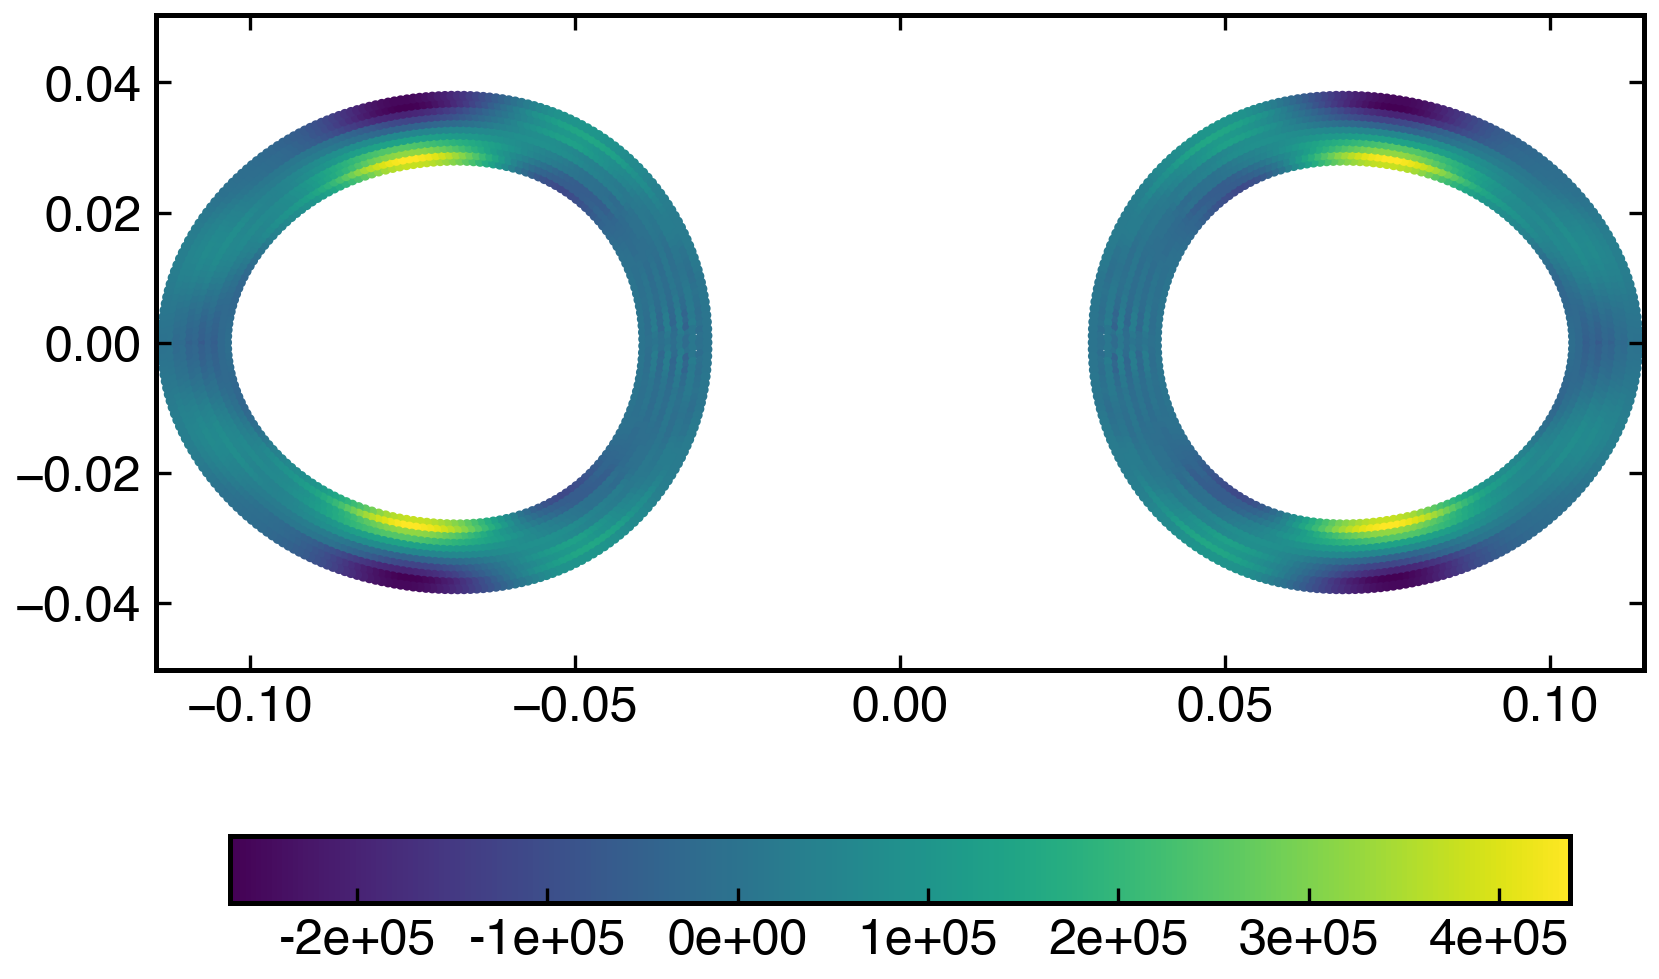
\includegraphics[width=1.0\textwidth]{figures/csph/figures/yan_2021_colliding_rubber_rings/poisson_ratio_0_47/time5}
    \subcaption{t = $15.4$ ms}\label{fig:rings:ipst-nu-0.47-4}
  \end{subfigure}
  \caption{Snapshots of particle positions with color indicating the stress
    field ($\sigma_{xx}$) solved by the current solver.}
\label{fig:rings:new-ipst-nu-0-47}
\end{figure}
%

With these examples we have demonstrated that,
\begin{itemize}
\item the collision SPH formulation can eliminate the spurious interactions that
  arises on the bodies when modeling with the SPH method alone.
\item Friction modeling between the elastic solids can also be handled with
  the collision SPH formulation.
\item CTVF with a contact force model is able to handle collision between the
  bodies with high Poisson ratio.
\end{itemize}
